\section{Define and explain, in your own words, what an object-oriented application framework is
and illustrate it with a concrete example of a framework you know.}

An object-oriented framework differs from a standard application because some of its parts, which are the hot-spots or variation points, may have a different implementation for each framework instance, and are left incomplete until instantiation time. A framework models the behavior of a family of applications. Its design (or skeleton) represents the commonalities among the applications and the variabilities are provided by the hot-spots. It's all about reusability.\\

To define correctly an object-oriented application framework with your own word you should include these parts :
\begin{itemize}
\item Domain/class of software : has a well defined domain where it provides behavior.
\item Skeleton / design / high-level language : a common design shared by all customization.
\item Collaborate / co-operating : a description of the behavior at a high level of abstraction, defining how classes participating in the framework interact.
\item Reusable / abstract classes / customized / specialization : can be tailored to a concrete context.
\item Classes / partial implementation: reuse of code as well as reuse of design.
\end{itemize}

As an example, the framework JUnit. It's an incomplete application for testing piece of code. Here the hotspots are the tests that you write. It's a framework because the tests that you wrote are called by JUnit ("the Hollywood principle"). It is reusable because you can write tests for all kind of applications.

\section{Discuss why/how object-oriented application frameworks are good for software reuse.}
Frameworks are one of the best bets on Software Reuse because they allow you to reuse both design and implementation.
The high-level design is the main intellectual content of software, and frameworks are a way to reuse it.
\begin{quote}
"Interface design and functional factoring constitutes the key intellectual content of software and are far more difficult to create or re-create than code." - Peter Deutsch
\end{quote}

A framework is just a partial application with holes. These holes are where you put your specialisation code. You can also add application specific code .

\section{Explain, and illustrate with a concrete example, the principle of inversion of control (also
known as the Hollywood principle) when building object-oriented application frameworks.}
The principle of inversion control (a.k.a the Hollywood principle) says this : “Don’t call us, we’ll call you”.
It means that, when using a framework, the application-specific code written by the programmer gets called by the framework and not in the other way like in a library.\\

Frameworks are partial applications  and thus (usually) define interaction patterns. Thus they insist on defining the flow of control.

For example, this simple python application which is a GUI, is a very simple example of inversion of control. The idea is that you write a function, but you never call it. Instead, you hand it over to another program and tell that program when to call it. Then you give control to that program.
\begin{lstlisting}[language=python]
import Tkinter

class App(object):
    def __init__(self, master):
        frame = Tkinter.Frame(master)
        frame.pack()

        self.button = Tkinter.Button(frame, text="QUIT", fg="red", command=frame.quit)
        self.button.pack(side=Tkinter.LEFT)

        self.hi_there = Tkinter.Button(frame, text="Hello", command=self.say_hi)
        self.hi_there.pack(side=Tkinter.LEFT)

    def say_hi(self):
        print "hi there, everyone!"

root = Tkinter.Tk()
app = App(root)

root.mainloop()
\end{lstlisting}

With "\texttt{class App(object)}" we start with a class definition, which will hold our callbacks and pass them to the appropriate parts of what I'll call the "master program".\\

With "\texttt{root = Tkinter.Tk()}" and "\texttt{app = App(root)}", we invoke our class, creating an instance. We create the root window, and then create an \texttt{App} instance with \texttt{root} as its parent.\\

Finally, with "\texttt{root.mainloop()}" pass control to Tkinter, which does the rest of the work.\\

source : http://stackoverflow.com/questions/6389248/could-anyone-give-a-simple-python-for-explaining-the-hollywood-principle-inver
\section{What distinguishes an object-oriented application framework from a library?}
What distinguishes an object-oriented application framework from a library is the Hollywood Principle seen above.

When using a library, the application calls the library, but the library is not aware of the application.

When using a framework, the application-specific code written by the programmer gets called by the framework.

\begin{center}
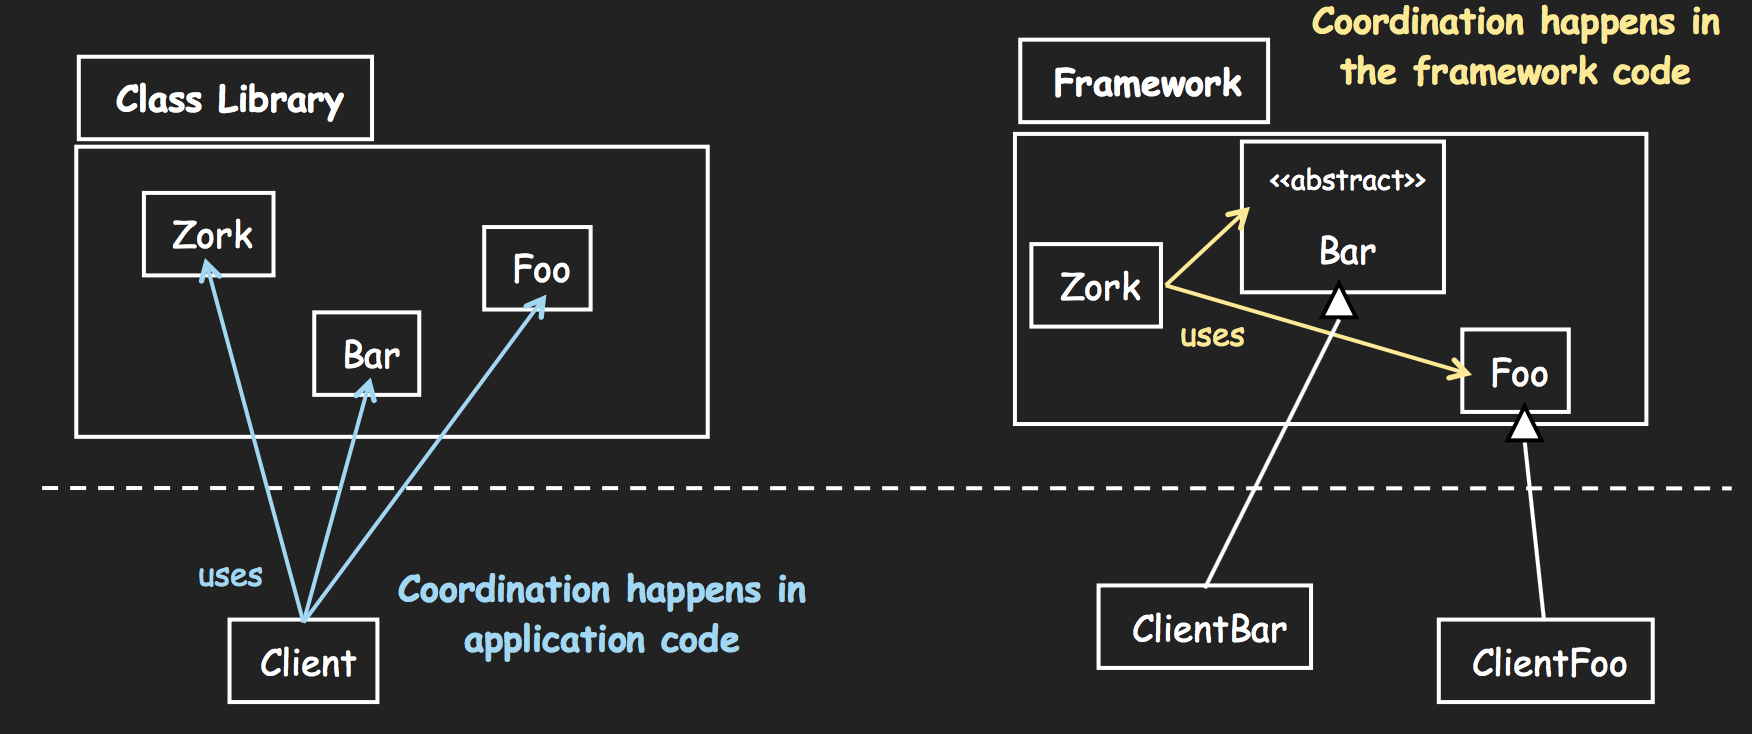
\includegraphics[scale=0.4]{libraryVSFramework.png}
\end{center}

\section{What is a hotspot in a framework? Explain and illustrate schematically.}
It's a "separate code that changes from the code that doesn't". Hotspots are the "holes" of a framework. These holes are code points where specialization code can alter behavior or add behavior to the framework. They're also known as hooks, hook methods or variation points.
As explained before, commonalities are common features between all the application in the family and variabilities are the specific features of some of the application in the family. The framework code defines the commonalities and the hotspots allow for a programmer to define the variabilities.

There is two kinds of hotspots : 
\begin{itemize}
\item Hotspots based upon inheritance : Filling in hotspots by specializing abstract  classes, method and interfaces (see slide 8A-19 for representation).
\item Hotspots based upon composition : Filling in parameters or objects by prefabricated components (see slide 8A-20 for representation).
\end{itemize}

\section{What types of frameworks can be distinguished?
What are the main differences between each of these types?}
There are three types of frameworks :
\begin{itemize}
\item White-box frameworks :
\begin{itemize}
\item Customisation through inheritance
\item Require insight in (and access to) implementation
\item \enquote{Easier} to design
\item More difficult to learn
\item More programming required for application development 
\item More flexibility
\end{itemize}
\item Black-box frameworks :
\begin{itemize}
\item Customisation through composition
\item Require insight in provided components
\item \enquote{Harder} to design
\item \enquote{Easier} to learn
\item Less programming required for application development 
\item Limited flexibility (no unanticipated variations)
\end{itemize}
\item Grey-box frameworks :  Grey box frameworks attempt to realize the benefits of both white and black box designs, while trying to avoid the perceived limitations of both.
\end{itemize}

White and black box form the extreme boundaries of framework design and usage principles. Most frameworks live somewhere in between these two extremes. A successful framework may start its life as white box, maturing towards grey or even black in a number of revisions.

\section{Explain and illustrate the Template Method design pattern and its key importance in
implementing object-oriented application frameworks.}

\subsection{Intent}
Defines the skeleton of an algorithm in an operation, deferring some steps to subclasses. Template Method lets subclasses redefine certain steps of the algorithm without changing the algorithm's structure.
\subsection{Solution}
Break out primitive steps into separate methods in ancestor class. Then, construct method for basic algorithm in ancestor that calls the primitive methods. Finally, override the primitive methods in descendant classes to implement specific tasks.
\subsection{Consequences}
A fundamental technique for code reuse – particularly important in class libraries and frameworks to factor out common behavior.
Leads to inverted control structure called “Hollywood Principle”.
A primitive method in the ancestor may provide a default behavior that descendants may optionally override (called hook methods).
\subsection{Related Patterns}
\begin{itemize}
\item  Factory Method is a form of Template Method used to create families of related objects.
\item Strategy is an alternate choice when the behaviour needs to be specified or may vary at run-time.
\end{itemize}
\subsection{Key importance in OO application framework}
A hotspot (this concept is explained above) in an object-oriented framework is often implemented via a Template Method. The template method defines the skeleton of the hot spot and the variable parts are deferred to the so-called hook methods?
The template method is defined on a template class which is part of the framework and the hook methods are defined on hook classes. These hook classes are concrete subclasses of the template class that are provided by framework users to customize the framework.

\begin{center}
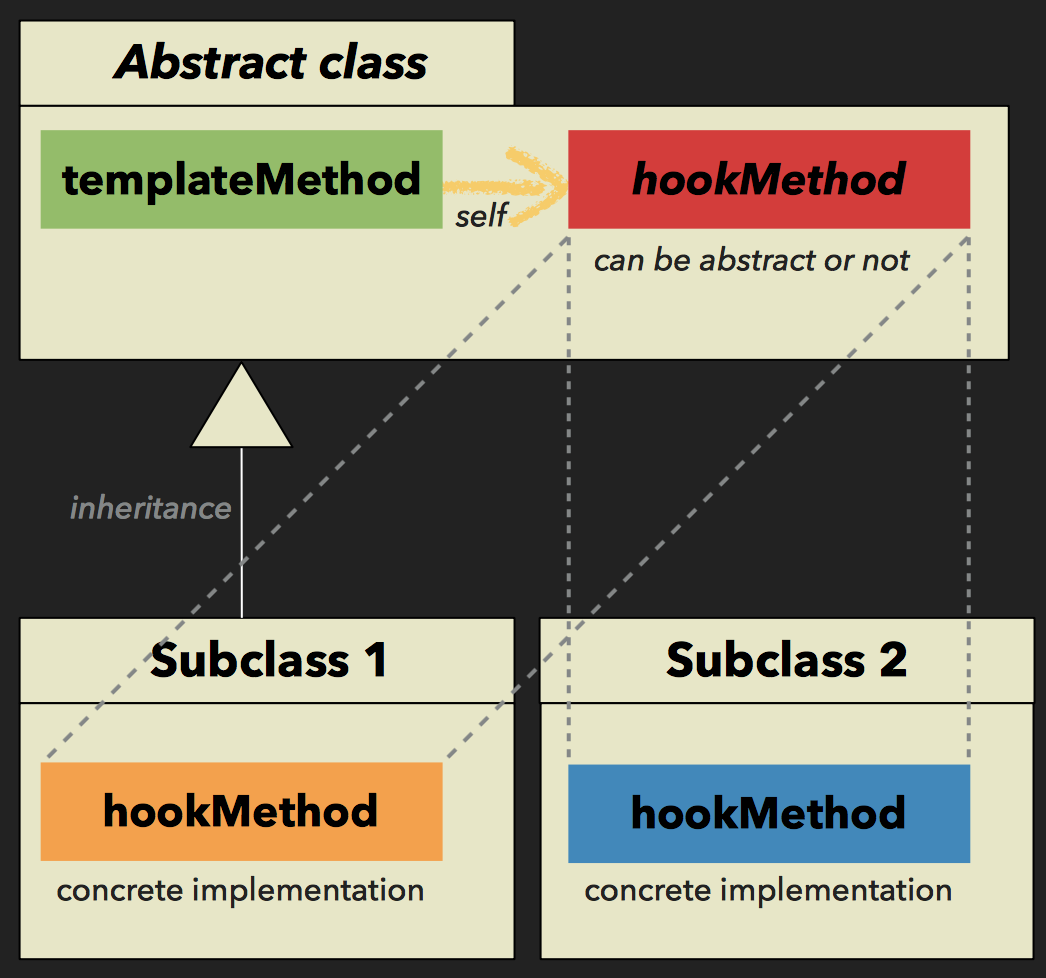
\includegraphics[scale=0.4]{template_method.png}
\end{center}